\documentclass[english]{article}\usepackage[]{graphicx}\usepackage[]{color}
%% maxwidth is the original width if it is less than linewidth
%% otherwise use linewidth (to make sure the graphics do not exceed the margin)
\makeatletter
\def\maxwidth{ %
  \ifdim\Gin@nat@width>\linewidth
    \linewidth
  \else
    \Gin@nat@width
  \fi
}
\makeatother

\definecolor{fgcolor}{rgb}{0.345, 0.345, 0.345}
\newcommand{\hlnum}[1]{\textcolor[rgb]{0.686,0.059,0.569}{#1}}%
\newcommand{\hlstr}[1]{\textcolor[rgb]{0.192,0.494,0.8}{#1}}%
\newcommand{\hlcom}[1]{\textcolor[rgb]{0.678,0.584,0.686}{\textit{#1}}}%
\newcommand{\hlopt}[1]{\textcolor[rgb]{0,0,0}{#1}}%
\newcommand{\hlstd}[1]{\textcolor[rgb]{0.345,0.345,0.345}{#1}}%
\newcommand{\hlkwa}[1]{\textcolor[rgb]{0.161,0.373,0.58}{\textbf{#1}}}%
\newcommand{\hlkwb}[1]{\textcolor[rgb]{0.69,0.353,0.396}{#1}}%
\newcommand{\hlkwc}[1]{\textcolor[rgb]{0.333,0.667,0.333}{#1}}%
\newcommand{\hlkwd}[1]{\textcolor[rgb]{0.737,0.353,0.396}{\textbf{#1}}}%

\usepackage{framed}
\makeatletter
\newenvironment{kframe}{%
 \def\at@end@of@kframe{}%
 \ifinner\ifhmode%
  \def\at@end@of@kframe{\end{minipage}}%
  \begin{minipage}{\columnwidth}%
 \fi\fi%
 \def\FrameCommand##1{\hskip\@totalleftmargin \hskip-\fboxsep
 \colorbox{shadecolor}{##1}\hskip-\fboxsep
     % There is no \\@totalrightmargin, so:
     \hskip-\linewidth \hskip-\@totalleftmargin \hskip\columnwidth}%
 \MakeFramed {\advance\hsize-\width
   \@totalleftmargin\z@ \linewidth\hsize
   \@setminipage}}%
 {\par\unskip\endMakeFramed%
 \at@end@of@kframe}
\makeatother

\definecolor{shadecolor}{rgb}{.97, .97, .97}
\definecolor{messagecolor}{rgb}{0, 0, 0}
\definecolor{warningcolor}{rgb}{1, 0, 1}
\definecolor{errorcolor}{rgb}{1, 0, 0}
\newenvironment{knitrout}{}{} % an empty environment to be redefined in TeX

\usepackage{alltt}
\usepackage[T1]{fontenc}
\usepackage[latin9]{inputenc}
\usepackage[margin=3cm]{geometry}
\geometry{verbose,tmargin=3cm,bmargin=3cm,lmargin=2.5cm,rmargin=2.5cm}
\setcounter{secnumdepth}{0}
\setcounter{tocdepth}{0}
\usepackage{url, indentfirst}
\usepackage{tabularx, booktabs, multirow, array, caption, color, longtable}
\usepackage{graphicx, fancyhdr, babel, xcolor, csquotes}
\usepackage{hyperref, lineno, setspace, pdflscape}
\usepackage[round]{natbib}
\graphicspath{ {C:/Users/jelber2/Dropbox/LSU/Dissertation/Manuscripts/immunome_2014/rnw/} }

\singlespacing

\title{Supporting Information for: \\
Elbers JP, Clostio RW and Taylor SS (2016) Population genetic \\
inferences using immune gene SNPs mirror patterns \\
inferred by microsatellites. Molecular Ecology Resources.}
\date{}
\author{}
\IfFileExists{upquote.sty}{\usepackage{upquote}}{}
\begin{document}

\maketitle



\noindent
\textbf{Table S1} Sequencing metrics for \textit{Gopherus polyphemus} samples. Percent UR for percent of total reads that were unique, Percent URA for percent of unique reads that were alignable, Mean coverage for mean number of reads across the target region, Percent 20x for percent of bases in target region with greater than 20x coverage, No. genes for number of genes, and No. exons for number of exons.\\
\begin{table}[ht]
\centering
\begin{tabular}{rcccccccc}
  \hline
 & Sample & Total reads & Percent UR & Percent URA & Mean coverage & Percent 20x & No. genes & No. exons \\ 
  \hline
1 & AL102 & 3,212,450 & 42.5489 & 98.7624 & 64.702327 & 70.9051 & 592 & 4,107 \\ 
  2 & AL103 & 4,465,410 & 41.6559 & 98.7366 & 86.236747 & 74.194 & 598 & 4,238 \\ 
  3 & AL106 & 3,359,715 & 45.6208 & 98.8027 & 71.663432 & 71.6972 & 600 & 4,156 \\ 
  4 & AL108 & 2,819,070 & 46.9525 & 98.4416 & 61.437226 & 72.4334 & 600 & 4,222 \\ 
  5 & FL846 & 3,053,761 & 48.2949 & 98.7728 & 68.408722 & 69.2006 & 594 & 4,120 \\ 
  6 & FL855 & 3,001,641 & 49.9861 & 98.8119 & 70.02287 & 70.426 & 587 & 4,162 \\ 
  7 & FL857 & 4,126,014 & 48.3302 & 98.7755 & 91.599757 & 73.6741 & 595 & 4,209 \\ 
  8 & FL880 & 2,495,515 & 47.5824 & 98.5998 & 55.003413 & 67.7526 & 592 & 4,140 \\ 
  9 & GA1044 & 2,735,000 & 50.4835 & 98.8161 & 64.467663 & 69.2348 & 594 & 4,135 \\ 
  10 & GA1435 & 3,114,664 & 48.0062 & 98.8188 & 69.54348 & 69.2231 & 593 & 4,088 \\ 
  11 & GA1835 & 3,160,564 & 47.5032 & 98.8015 & 69.893149 & 70.4834 & 595 & 4,135 \\ 
  12 & GA462 & 1,692,328 & 50.9997 & 98.7798 & 40.600786 & 61.147 & 586 & 3,934 \\ 
  13 & LA62 & 2,490,648 & 47.5604 & 98.7996 & 55.582373 & 67.2087 & 592 & 4,032 \\ 
  14 & LA66 & 2,366,268 & 48.6917 & 98.6262 & 53.254455 & 65.3586 & 592 & 3,992 \\ 
  15 & LA77 & 3,449,116 & 46.1951 & 98.7934 & 74.612173 & 72.2789 & 600 & 4,162 \\ 
  16 & LA78 & 1,920,641 & 55.6212 & 98.8716 & 50.102979 & 63.859 & 596 & 3,899 \\ 
   \hline
\end{tabular}
\end{table}

\pagebreak{}
\begin{longtable}{l}
\noindent
\textbf{Table S2} All genes with di-allelic, polymorphic SNPs from 16 \textit{Gopherus polyphemus} samples.\\
\hline
\textbf{Gene}\\
\hline
\endfirsthead
\multicolumn{1}{l}
{Table S2 -- \textit{Continued from previous page}} \\
\hline
\textbf{Gene}\\
\hline
\endhead
\hline \multicolumn{1}{r}{\textit{Continued on next page}} \\
\endfoot
\hline
\endlastfoot
1-phosphatidylinositol 4,5-bisphosphate phosphodiesterase gamma-1-like \\ 
16 kDa beta-galactoside-binding lectin-like \\ 
25-hydroxyvitamin D-1 alpha hydroxylase, mitochondrial \\ 
3-phosphoinositide dependent protein kinase 1 \\ 
4-hydroxy-2-oxoglutarate aldolase 1 \\ 
A.superbus venom factor 1-like \\ 
acetylcholinesterase-like \\ 
active BCR-related \\ 
adenosine A2b receptor \\ 
adenosine A3 receptor \\ 
ADP-ribosylation factor-like 13B \\ 
alpha-2-macroglobulin \\ 
alpha-2-macroglobulin-like \\ 
alpha-2-macroglobulin-like 1 \\ 
alpha-2-macroglobulin-like protein 1 \\ 
angiogenin-2-like \\ 
ankyrin repeat and death domain containing 1A \\ 
annexin A3 \\ 
antigen-presenting glycoprotein CD1d1-like \\ 
apolipoprotein A-IV \\ 
apoptosis-associated speck-like protein containing a CARD \\ 
aquaporin 4 \\ 
arrestin, beta 2 \\ 
ATPase, Cu++ transporting, alpha polypeptide \\ 
autophagy related 5 \\ 
B-cell CLL/lymphoma 10 \\ 
B-cell CLL/lymphoma 2 \\ 
B-cell CLL/lymphoma 3 \\ 
B-cell receptor-associated protein 29 \\ 
B-cell receptor-associated protein 31 \\ 
B-cell scaffold protein with ankyrin repeats 1 \\ 
B and T lymphocyte associated \\ 
B lymphoid tyrosine kinase \\ 
bactericidal permeability-increasing protein-like \\ 
bactericidal/permeability-increasing protein \\ 
basic leucine zipper transcription factor, ATF-like \\ 
beta-2-microglobulin \\ 
bone morphogenetic protein 6 \\ 
bone morphogenetic protein receptor, type IA \\ 
breakpoint cluster region \\ 
butyrophilin-like protein 9 \\ 
butyrophilin subfamily 1 member A1-like \\ 
butyrophilin subfamily 2 member A1-like \\ 
butyrophilin subfamily 3 member A2-like \\ 
butyrophilin subfamily 3 member A3-like \\ 
C-C chemokine receptor type 5-like \\ 
C-C motif chemokine 5-like \\ 
C-type lectin domain family 1 member A-like \\ 
C-type lectin domain family 2 member B-like \\ 
C-type lectin domain family 2 member D-like \\ 
C-type lectin domain family 4 member D-like \\ 
C-type lectin domain family 4 member E-like \\ 
C-type lectin domain family 4 member G-like \\ 
C-X-C motif chemokine 10-like \\ 
C3a anaphylatoxin chemotactic receptor-like \\ 
C4b-binding protein alpha chain-like \\ 
C5a anaphylatoxin chemotactic receptor 1-like \\ 
cactin, spliceosome C complex subunit \\ 
calcium binding and coiled-coil domain 2 \\ 
calcium channel, voltage-dependent, beta 3 subunit \\ 
calcium channel, voltage-dependent, beta 4 subunit \\ 
calcium/calmodulin-dependent protein kinase IV \\ 
calicin \\ 
cardiotrophin-like cytokine factor 1 \\ 
caspase recruitment domain family, member 9 \\ 
cathepsin G-like \\ 
Cbl proto-oncogene B, E3 ubiquitin protein ligase \\ 
CD14 molecule \\ 
CD180 molecule \\ 
CD226 molecule \\ 
CD247 molecule \\ 
CD274 molecule \\ 
CD36 molecule (thrombospondin receptor) \\ 
CD37 molecule \\ 
CD3e molecule, epsilon (CD3-TCR complex) \\ 
CD40 molecule, TNF receptor superfamily member 5 \\ 
CD74 molecule, major histocompatibility complex, class II invariant chain \\ 
CD79a molecule, immunoglobulin-associated alpha \\ 
CD79b molecule, immunoglobulin-associated beta \\ 
CD82 molecule \\ 
cell adhesion molecule 1 \\ 
cell adhesion molecule 4 \\ 
cell division cycle 37 \\ 
cell division cycle 37-like 1 \\ 
centromere protein F, 350/400kDa \\ 
chemokine (C-C motif) receptor 7 \\ 
chemokine (C-X3-C motif) receptor 1 \\ 
chromosome unknown open reading frame, human C9orf84 \\ 
cis-aconitate decarboxylase-like \\ 
class I histocompatibility antigen, F10 alpha chain-like \\ 
class II histocompatibility antigen, M alpha chain \\ 
class II, major histocompatibility complex, transactivator \\ 
coagulation factor II (thrombin) receptor-like 1 \\ 
coagulation factor XIII, B polypeptide \\ 
coenzyme Q10 homolog B (S. cerevisiae) \\ 
coiled-coil domain containing 142 \\ 
coiled-coil domain containing 151 \\ 
coiled-coil domain containing 170 \\ 
collagen, type III, alpha 1 \\ 
collectin-46-like \\ 
collectin sub-family member 12 \\ 
complement C1r-B subcomponent-like \\ 
complement C2-like \\ 
complement C3-like \\ 
complement component 1, q subcomponent binding protein \\ 
complement component 1, q subcomponent, A chain \\ 
complement component 1, r subcomponent \\ 
complement component 1, s subcomponent \\ 
complement component 8, alpha polypeptide \\ 
complement decay-accelerating factor-like \\ 
complement factor B \\ 
complement factor H \\ 
complement factor properdin \\ 
complement receptor type 2-like \\ 
CUB and Sushi multiple domains 1 \\ 
cyclic GMP-AMP synthase-like \\ 
cytochrome P450 27C1 \\ 
cytotoxic and regulatory T cell molecule \\ 
cytotoxic T-lymphocyte-associated protein 4 \\ 
DEAD (Asp-Glu-Ala-Asp) box polypeptide 58 \\ 
death-associated protein kinase 1 \\ 
death-associated protein kinase 2-like \\ 
death-associated protein kinase 3 \\ 
death-associated protein kinase 3-like \\ 
dedicator of cytokinesis 2 \\ 
dedicator of cytokinesis protein 2-like \\ 
DEXH (Asp-Glu-X-His) box polypeptide 58 \\ 
discs, large homolog 1 (Drosophila) \\ 
dispanin subfamily A member 2b \\ 
DLA class II histocompatibility antigen, DR-1 beta chain-like \\ 
DnaJ (Hsp40) homolog, subfamily A, member 3 \\ 
docking protein 6 \\ 
dual specificity phosphatase 10 \\ 
duodenase-1-like \\ 
dynactin 1 \\ 
E3 ubiquitin-protein ligase TRIM39-like \\ 
E3 ubiquitin-protein ligase TRIM39 pseudogene \\ 
E3 ubiquitin-protein ligase TRIM56-like \\ 
eomesodermin \\ 
epiregulin \\ 
excision repair cross-complementation group 1 \\ 
exonuclease 1 \\ 
exosome component 3 \\ 
extracellular matrix protein 1 \\ 
family with sequence similarity 105, member A \\ 
family with sequence similarity 177, member A1 \\ 
family with sequence similarity 83, member E \\ 
Fanconi anemia, complementation group F \\ 
Fas cell surface death receptor \\ 
Fc fragment of IgE, high affinity I, receptor for; gamma polypeptide \\ 
feline Gardner-Rasheed sarcoma viral oncogene homolog \\ 
feline sarcoma oncogene \\ 
fer (fps/fes related) tyrosine kinase \\ 
ficolin-1-like \\ 
ficolin-2-like \\ 
ficolin (collagen/fibrinogen domain containing) 3 \\ 
fucokinase \\ 
FYN oncogene related to SRC, FGR, YES \\ 
G-protein coupled receptor 183-like \\ 
G patch domain and KOW motifs \\ 
gastrula zinc finger protein XlCGF57.1-like \\ 
GATA binding protein 3 \\ 
glucosaminyl (N-acetyl) transferase 3, mucin type \\ 
glutamyl-prolyl-tRNA synthetase \\ 
glutathione peroxidase 1 \\ 
glutathione peroxidase 2 (gastrointestinal) \\ 
glycosylphosphatidylinositol specific phospholipase D1 \\ 
granzyme-like protein 2 \\ 
GRB2-associated binding protein 2 \\ 
growth arrest-specific 6 \\ 
GTP cyclohydrolase 1 \\ 
GTP cyclohydrolase 1-like \\ 
H-2 class II histocompatibility antigen, A-R alpha chain-like \\ 
H-2 class II histocompatibility antigen, E-S beta chain-like \\ 
H2.0-like homeobox \\ 
heat shock 60kDa protein 1 (chaperonin) \\ 
hemopexin \\ 
heparan sulfate (glucosamine) 3-O-sulfotransferase 4 \\ 
HLA class II histocompatibility antigen, DP alpha 1 chain-like \\ 
HLA class II histocompatibility antigen, DR alpha chain-like \\ 
HLA class II histocompatibility antigen, DR beta 5 chain-like \\ 
HLA class II histocompatibility antigen, DRB1-15 beta chain-like \\ 
immunoresponsive 1 homolog (mouse) \\ 
importin 11 \\ 
indoleamine 2,3-dioxygenase 1 \\ 
inositol polyphosphate-5-phosphatase, 145kDa \\ 
insulin-like growth factor 1 receptor \\ 
integrin alpha-L-like \\ 
interferon-induced guanylate-binding protein 1 \\ 
interferon-induced guanylate-binding protein 1-like \\ 
interferon-induced protein 44-like \\ 
interferon-induced protein with tetratricopeptide repeats 1-like \\ 
interferon-induced protein with tetratricopeptide repeats 5 \\ 
interferon induced transmembrane protein 5 \\ 
interferon kappa-like \\ 
interferon regulatory factor 3 \\ 
interferon regulatory factor 7 \\ 
interferon regulatory factor 8 \\ 
interferon, kappa \\ 
interleukin-1 receptor-associated kinase 1 \\ 
interleukin-36 receptor antagonist protein \\ 
interleukin 1 receptor-like 1 \\ 
interleukin 12 receptor, beta 1 \\ 
interleukin 12A \\ 
interleukin 12B \\ 
interleukin 18 \\ 
interleukin 18 receptor 1 \\ 
interleukin 20 receptor beta \\ 
interleukin 23 receptor \\ 
interleukin 27 receptor, alpha \\ 
interleukin 4 receptor \\ 
interleukin 6 \\ 
interleukin 7 receptor \\ 
ISG15 ubiquitin-like modifier \\ 
Janus kinase 2 \\ 
Janus kinase 3 \\ 
kelch-like family member 24 \\ 
kelch-like family member 35 \\ 
kelch-like family member 38 \\ 
kelch-like family member 6 \\ 
kelch repeat and BTB (POZ) domain containing 8 \\ 
keratin, type II cytoskeletal 1-like \\ 
killer cell lectin-like receptor subfamily B member 1B allele C \\ 
killer cell lectin-like receptor subfamily F member 1 \\ 
killer cell lectin-like receptor subfamily G member 1 \\ 
kynureninase \\ 
lectin, galactoside-binding, soluble, 2 \\ 
lectin, galactoside-binding, soluble, 8 \\ 
leucine rich repeat (in FLII) interacting protein 2 \\ 
leucine rich repeat containing 70 \\ 
lymphocyte-specific protein tyrosine kinase \\ 
lymphocyte cytosolic protein 1 (L-plastin) \\ 
lymphotoxin alpha \\ 
lysosomal trafficking regulator \\ 
Mab-21 domain containing 1 \\ 
macrophage migration inhibitory factor \\ 
major histocompatibility complex class I-related gene protein-like \\ 
mannan-binding lectin serine peptidase 1  \\ 
mannan-binding lectin serine peptidase 2 \\ 
mast cell protease 1A-like \\ 
mast cell protease 3-like \\ 
mediator of RNA polymerase II transcription subunit 1-like \\ 
melanotransferrin-like \\ 
membrane-associated ring finger (C3HC4) 1, E3 ubiquitin protein ligase \\ 
membrane cofactor protein-like \\ 
mitochondrial carrier 2 \\ 
mitogen-activated protein kinase-activated protein kinase 2 \\ 
mitogen-activated protein kinase kinase 7 \\ 
mitogen-activated protein kinase kinase kinase 14 \\ 
mothers against decapentaplegic homolog 6-like \\ 
mucosa-associated lymphoid tissue lymphoma translocation protein 1-like \\ 
mucosa associated lymphoid tissue lymphoma translocation gene 1 \\ 
mutL homolog 1 \\ 
mutS homolog 6 \\ 
myelin-oligodendrocyte glycoprotein-like \\ 
myosin IF \\ 
myosin light chain, phosphorylatable, fast skeletal muscle \\ 
N(alpha)-acetyltransferase 25, NatB auxiliary subunit \\ 
NACHT, LRR and PYD domains-containing protein 1-like \\ 
NACHT, LRR and PYD domains-containing protein 12-like \\ 
natural killer cells antigen CD94-like \\ 
NCK-associated protein 1-like \\ 
Nedd4 family interacting protein 1 \\ 
negative regulator of ubiquitin-like proteins 1 \\ 
NK2 homeobox 3 \\ 
NLR family member X1 \\ 
NLR family, CARD domain containing 5 \\ 
nuclear factor of activated T-cells, cytoplasmic 2-like \\ 
nuclear fac. of kappa light polypep. gene enhancer in B-cells 2 (p49/p100) \\ 
nuclear fac. of kappa light polypep. gene enhancer in B-cells inhibitor, alpha \\ 
olfactomedin-4-like \\ 
olfactomedin-like \\ 
olfactomedin 4 \\ 
oncoprotein induced transcript 3 \\ 
opioid receptor, kappa 1 \\ 
OTU deubiquitinase 7B \\ 
OTU deubiquitinase with linear linkage specificity \\ 
ovostatin-like \\ 
paired amphipathic helix protein Sin3a-like \\ 
PAX interacting (with transcription-activation domain) protein 1 \\ 
peptidase domain containing associated with muscle regeneration 1 \\ 
peptidoglycan recognition protein 2 \\ 
peptidoglycan recognition protein 3-like \\ 
peroxisome proliferator-activated receptor gamma \\ 
phosphatidylinositol 4-kinase type 2 alpha \\ 
phosphodiesterase 4B, cAMP-specific \\ 
phosphodiesterase 4C, cAMP-specific \\ 
phosphodiesterase 4D, cAMP-specific \\ 
phosphoinositide-3-kinase adaptor protein 1 \\ 
phospholipase A2, group IB (pancreas) \\ 
phospholipase A2, minor isoenzyme-like \\ 
phospholipase C, gamma 1 \\ 
phospholipase D2-like \\ 
phospholipid scramblase 2 \\ 
phospholipid scramblase family, member 5 \\ 
pleckstrin hom. domain contain., family A (phosphoinositide bind. spec.) member 1 \\ 
poliovirus receptor-related 2 (herpesvirus entry mediator B) \\ 
poly (ADP-ribose) polymerase family, member 9 \\ 
poly [ADP-ribose] polymerase 9-like \\ 
polymerase (RNA) III (DNA directed) polypeptide C (62kD) \\ 
polymerase (RNA) III (DNA directed) polypeptide D, 44kDa \\ 
polymerase (RNA) III (DNA directed) polypeptide F, 39 kDa \\ 
polymerase (RNA) III (DNA directed) polypeptide G (32kD) \\ 
polymerase (RNA) III (DNA directed) polypeptide G (32kD)-like \\ 
potassium channel tetramerization domain containing 7 \\ 
POU class 2 homeobox 2 \\ 
presenilin 2 \\ 
programmed cell death 1 ligand 2-like \\ 
proteasome (prosome, macropain) subunit, beta type, 4 \\ 
protein kinase C, beta \\ 
protein kinase C, delta \\ 
protein kinase C, epsilon \\ 
protein kinase C, theta \\ 
protein kinase C, zeta \\ 
protein kinase D2 \\ 
protein phosphatase 2, regulatory subunit B\&apos;\&apos;, gamma \\ 
protein phosphatase 3, catalytic subunit, beta isozyme \\ 
protein tyrosine phosphatase, non-receptor type 2 \\ 
protein tyrosine phosphatase, non-receptor type 22 (lymphoid) \\ 
protein tyrosine phosphatase, non-receptor type 6 \\ 
protein tyrosine phosphatase, receptor type, C \\ 
protein tyrosine phosphatase, receptor type, N polypeptide 2 \\ 
purine nucleoside phosphorylase \\ 
purinergic receptor P2X, ligand-gated ion channel, 7 \\ 
pyroglutamyl-peptidase I-like \\ 
RAB guanine nucleotide exchange factor (GEF) 1 \\ 
RAB17, member RAS oncogene family \\ 
RAB27A, member RAS oncogene family \\ 
RanBP-type and C3HC4-type zinc finger containing 1 \\ 
rano class II histocompatibility antigen, A beta chain-like \\ 
RAR-related orphan receptor C \\ 
RAS guanyl releasing protein 1 (calcium and DAG-regulated) \\ 
receptor-interacting serine-threonine kinase 2 \\ 
receptor-interacting serine/threonine-protein kinase 2-like \\ 
regulator of cell cycle \\ 
retinoic acid receptor, alpha \\ 
Rho guanine nucleotide exchange factor (GEF) 37 \\ 
RIB43A domain with coiled-coils 1 \\ 
ribonuclease-like \\ 
ribosomal protein L13a \\ 
ribosomal protein S6 kinase, 90kDa, polypeptide 3 \\ 
ribosomal protein S6 kinase, 90kDa, polypeptide 6 \\ 
ring finger and CCCH-type domains 1 \\ 
ring finger and CCCH-type domains 2 \\ 
ring finger protein 135 \\ 
ring finger protein 19B \\ 
ring finger protein 31 \\ 
S100 calcium binding protein A14 \\ 
SAM and SH3 domain-containing protein 1 \\ 
SAM and SH3 domain containing 3 \\ 
SAM domain and HD domain 1 \\ 
SAM domain, SH3 domain and nuclear localization signals 1 \\ 
Sec61 alpha 1 subunit (S. cerevisiae) \\ 
sema domain, Ig, TM and short cytoplasmic domain, (semaphorin) 4A \\ 
sema domain, Ig, TM and short cytoplasmic domain, (semaphorin) 4B \\ 
semaphorin-7A-like \\ 
semaphorin 7A, GPI membrane anchor (John Milton Hagen blood group) \\ 
serine/threonine kinase 11 \\ 
serpin peptidase inhibitor, clade G (C1 inhibitor), member 1 \\ 
SH2 domain containing 1A \\ 
SH2 domain containing 1B \\ 
SH2B adaptor protein 2 \\ 
sialidase 2 (cytosolic sialidase) \\ 
signal transducer and activator of transcription 6, interleukin-4 induced \\ 
SIN3 transcription regulator family member A \\ 
sirtuin 1 \\ 
SMAD family member 6 \\ 
solute carrier family 26 (anion exchanger), member 6 \\ 
solute carrier family 26 (anion exchanger), member 8 \\ 
solute carrier family 26 (anion exchanger), member 9 \\ 
solute carrier family 26, member 10 \\ 
solute carrier family 30 (zinc transporter), member 8 \\ 
spinster homolog 1 (Drosophila) \\ 
spinster homolog 2 (Drosophila) \\ 
spinster homolog 3 (Drosophila) \\ 
spleen tyrosine kinase \\ 
src kinase associated phosphoprotein 1 \\ 
src kinase associated phosphoprotein 2 \\ 
steroidogenic acute regulatory protein \\ 
steroidogenic acute regulatory protein, mitochondrial-like \\ 
stomatin (EPB72)-like 2 \\ 
strawberry notch homolog 1 (Drosophila) \\ 
strawberry notch homolog 2 (Drosophila) \\ 
suppressor of cytokine signaling 5 \\ 
suppressor of cytokine signaling 5-like \\ 
suppressor of Ty 6 homolog (S. cerevisiae) \\ 
suppressor of variegation 3-9 homolog 1 (Drosophila) \\ 
SWAP switching B-cell complex 70kDa subunit \\ 
synaptotagmin binding, cytoplasmic RNA interacting protein \\ 
syntaxin 11 \\ 
syntaxin 19 \\ 
syntaxin binding protein 2 \\ 
syntaxin binding protein 3 \\ 
T-box 21 \\ 
TANK-binding kinase 1 \\ 
tec protein tyrosine kinase \\ 
tetraspanin 19 \\ 
thaicobrin-like \\ 
thrombospondin 1 \\ 
thymocyte selection associated \\ 
thymocyte selection associated family member 2 \\ 
TLR4 interactor with leucine-rich repeats \\ 
TNF receptor-associated factor 1-like \\ 
TNF receptor-associated factor 2 \\ 
TNF receptor-associated factor 3 \\ 
TNF receptor-associated factor 6, E3 ubiquitin protein ligase \\ 
TNFAIP3 interacting protein 2 \\ 
TNFAIP3 interacting protein 3 \\ 
toll-interleukin 1 receptor (TIR) domain containing adaptor protein \\ 
toll-like receptor 13 \\ 
toll-like receptor 2 \\ 
toll-like receptor 7 \\ 
toll-like receptor 8 \\ 
toll-like receptor adaptor molecule 1 \\ 
toll-like receptor adaptor molecule 2 \\ 
transferrin \\ 
transforming growth factor, beta 2 \\ 
transforming growth factor, beta 3 \\ 
transforming growth factor, beta receptor III \\ 
transforming growth factor, beta receptor III-like \\ 
transient receptor potential cation channel subfamily M member 4-like \\ 
transient receptor potential cation channel, subfamily M, member 4 \\ 
translation machinery associated 16 homolog (S. cerevisiae) \\ 
transmembrane protein 125 \\ 
transmembrane protein 167A \\ 
tripartite motif-containing protein 10-like \\ 
tripartite motif-containing protein 7-like \\ 
tripartite motif containing 56 \\ 
tumor necrosis factor (ligand) superfamily, member 13b \\ 
tumor necrosis factor receptor superfamily member 14-like \\ 
tumor necrosis factor receptor superfamily member 5-like \\ 
tumor necrosis factor receptor superfamily, member 14 \\ 
tumor necrosis factor, alpha-induced protein 3 \\ 
TXK tyrosine kinase \\ 
tyrosine 3-monooxygenase/tryptophan 5-monooxygenase activation protein, zeta \\ 
UBA domain containing 2 \\ 
unc-13 homolog D (C. elegans) \\ 
unc-93 homolog B1 (C. elegans) \\ 
uncharacterized LOC101938270 \\ 
uncharacterized LOC101938480 \\ 
uncharacterized LOC101940718 \\ 
uncharacterized LOC101941368 \\ 
uncharacterized LOC101944094 \\ 
uncharacterized LOC101945191 \\ 
uncharacterized LOC101945921 \\ 
uncharacterized LOC101945971 \\ 
uncharacterized LOC101948866 \\ 
uncharacterized LOC101948974 \\ 
uncharacterized LOC101949200 \\ 
uncharacterized LOC101949947 \\ 
uncharacterized LOC101950806 \\ 
uncharacterized LOC101950941 \\ 
uncharacterized LOC101950982 \\ 
uncharacterized LOC101951626 \\ 
uncharacterized LOC103305939 \\ 
uncharacterized LOC103305969 \\ 
uncharacterized LOC103305996 \\ 
uncharacterized LOC103306364 \\ 
uncharacterized LOC103306443 \\ 
uncharacterized LOC103306956 \\ 
uncharacterized LOC103307015 \\ 
uncharacterized protein-like \\ 
v-kit Hardy-Zuckerman 4 feline sarcoma viral oncogene homolog \\ 
v-rel avian reticuloendotheliosis viral oncogene homolog A \\ 
v-rel avian reticuloendotheliosis viral oncogene homolog B \\ 
v-yes-1 Yamaguchi sarcoma viral related oncogene homolog \\ 
vav 1 guanine nucleotide exchange factor \\ 
vav 3 guanine nucleotide exchange factor \\ 
VCP-interacting membrane protein \\ 
veficolin-1-like \\ 
venom factor-like \\ 
wingless-type MMTV integration site family, member 5A \\ 
Wiskott-Aldrich syndrome \\ 
X-ray repair complementing defective repair in Chinese hamster cells 4 \\ 
Z-DNA binding protein 1 \\ 
zeta-chain (TCR) associated protein kinase 70kDa \\ 
zinc-binding protein A33-like \\ 
zinc finger and BTB domain containing 41 \\ 
zinc finger protein 239-like \\ 
zinc finger protein 271-like \\ 
zinc finger protein 418-like \\ 
zinc finger protein 436-like \\ 
zinc finger protein 501-like \\ 
zinc finger protein 551-like \\ 
zinc finger protein 572-like \\ 
zinc finger protein 850-like \\ 
zinc finger protein 883-like \\ 
zinc finger protein RFP-like \\ 
zinc finger, SWIM-type containing 7 \\ 
zona pellucida sperm-binding protein 3-like \\ 
zona pellucida sperm-binding protein 4-like \\ 
\hline
\end{longtable}

\pagebreak{}
\noindent
\begin{knitrout}
\definecolor{shadecolor}{rgb}{0.969, 0.969, 0.969}\color{fgcolor}
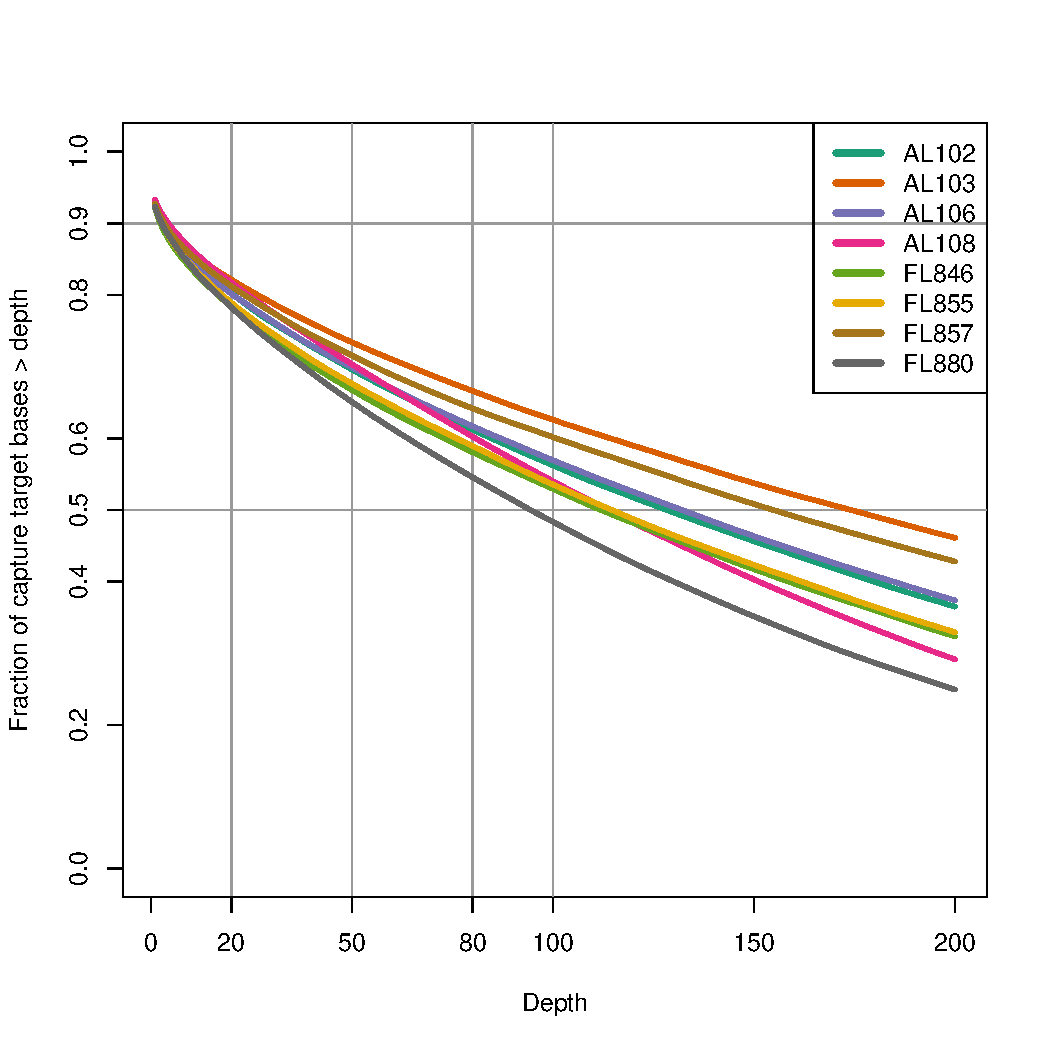
\includegraphics[width=\maxwidth]{figure/Figure-2-1} 

\end{knitrout}
\noindent
\textbf{Fig. S1} Coverage plots for first eight \textit{Gopherus polyphemus} samples showing number of sequencing reads at or above specified proportions. A value at 100 Depth and 0.5 fraction means 50 percent of bases were at or above 100X coverage.\\


\pagebreak{}
\noindent
\begin{knitrout}
\definecolor{shadecolor}{rgb}{0.969, 0.969, 0.969}\color{fgcolor}
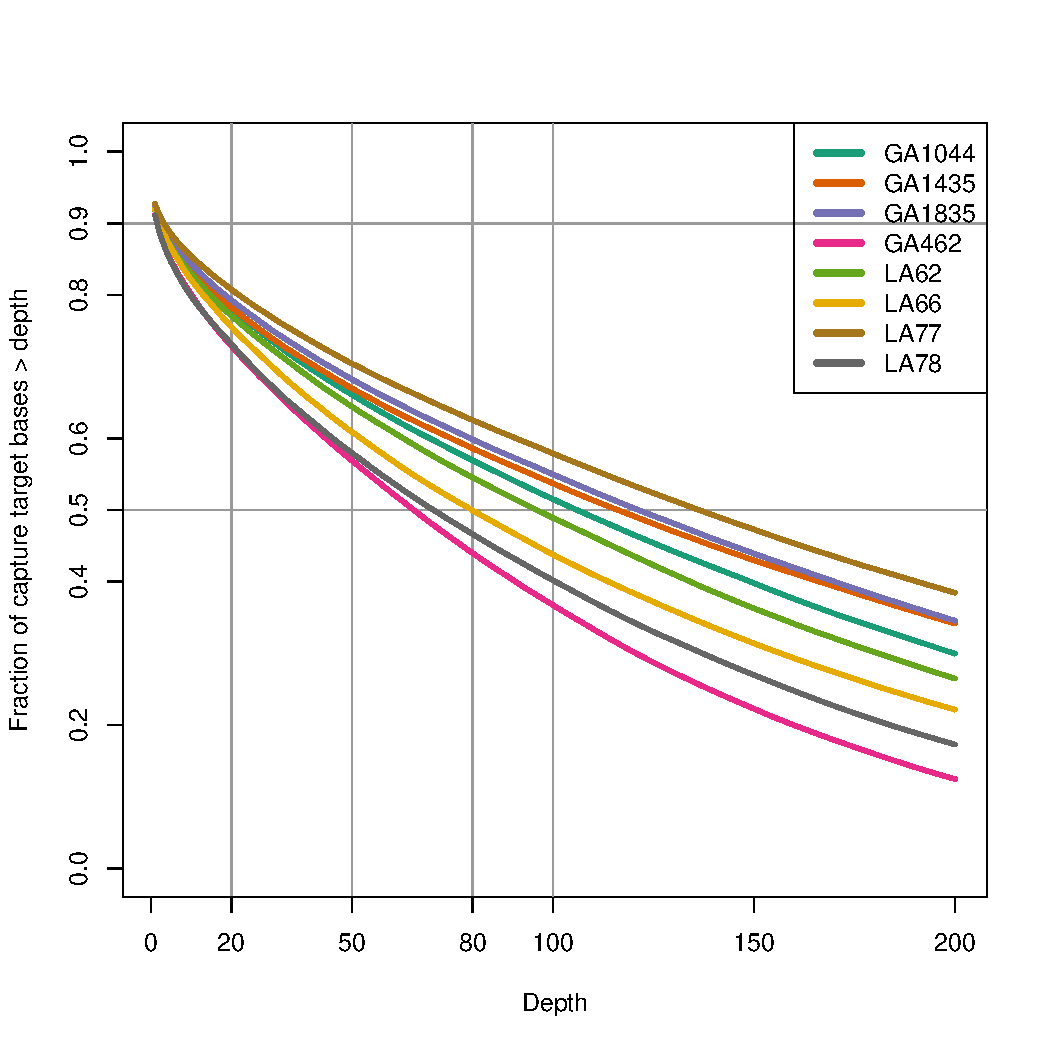
\includegraphics[width=\maxwidth]{figure/Figure-3-1} 

\end{knitrout}
\noindent
\textbf{Fig. S2} Coverage plots for last eight \textit{Gopherus polyphemus} samples showing number of sequencing reads at or above specified proportions.\\


\pagebreak{}
\noindent
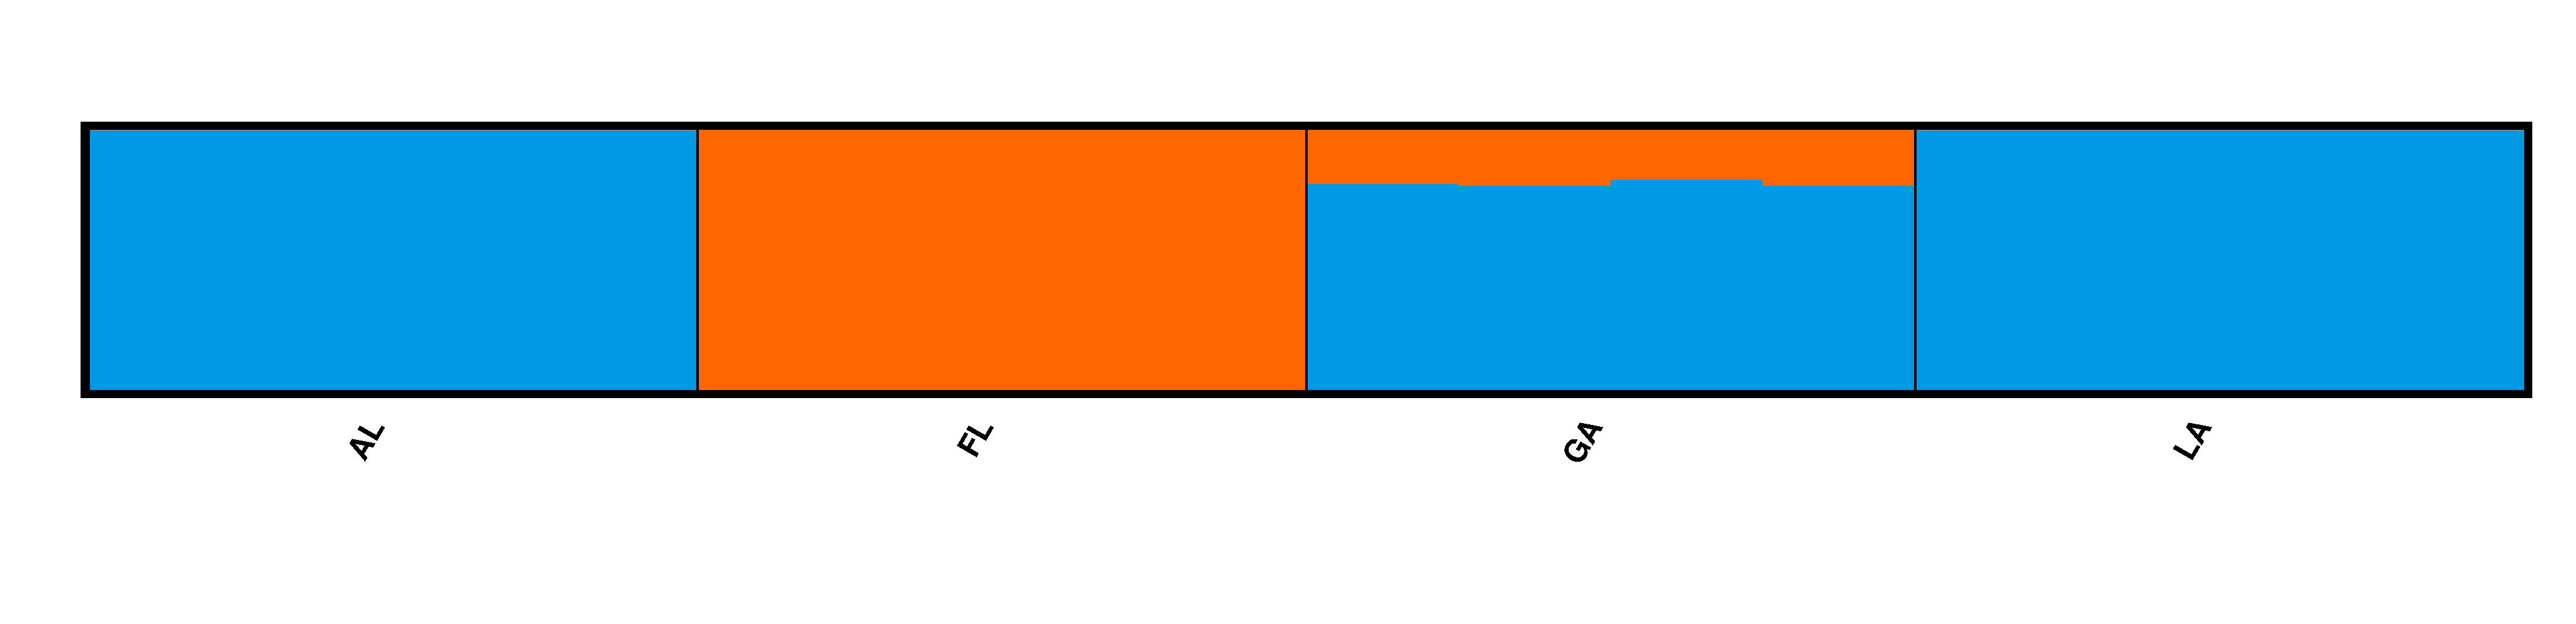
\includegraphics [scale=1.0]{K2MajorCluster-snps}
\noindent
\textbf{Fig. S3} \texttt{STRUCTURE} plot for 16 \textit{Gopherus polyphemus} sequenced at 17,901 immune gene SNPs with optimum number of clusters \textit{K} = 2 determined by \texttt{STRUCTURE HARVESTER}.\\

\pagebreak{}
\noindent
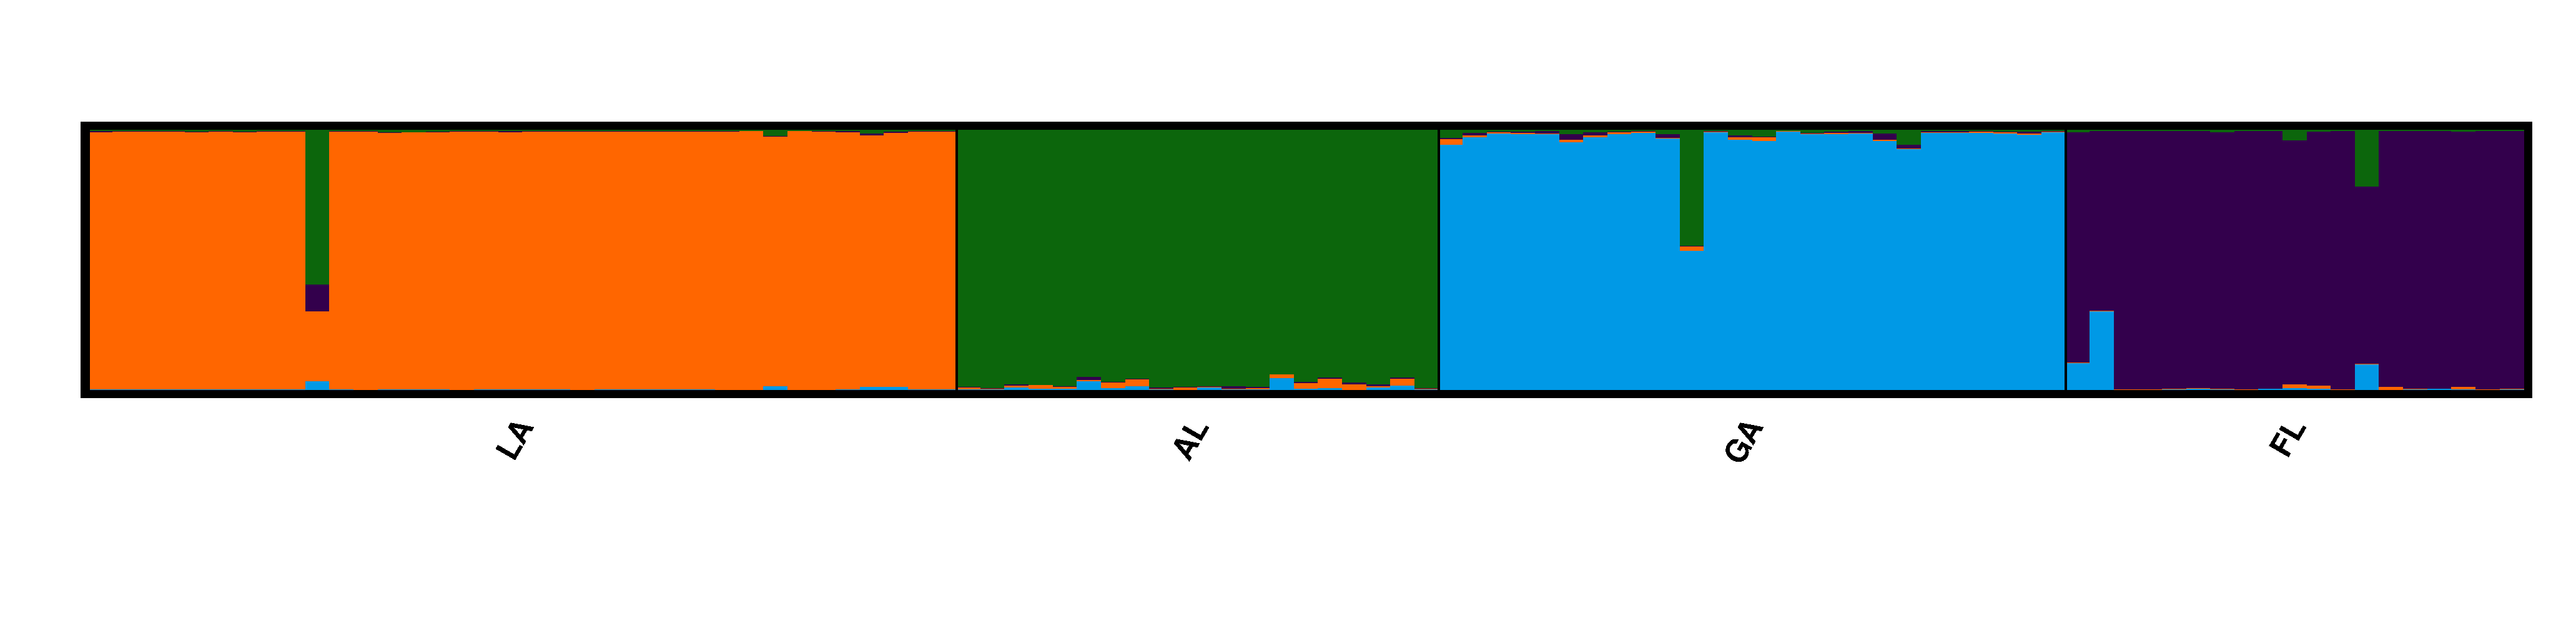
\includegraphics [scale=1.0]{structure-results-msats-review-clumpak-k4}
\noindent
\textbf{Fig. S4} \texttt{STRUCTURE} plot for the full microsatellite dataset (101 \textit{Gopherus polyphemus} genotyed at 10 microsatellite loci) with optimum number of clusters \textit{K} = 4 determined by \texttt{STRUCTURE HARVESTER}.\\

\pagebreak{}
\noindent
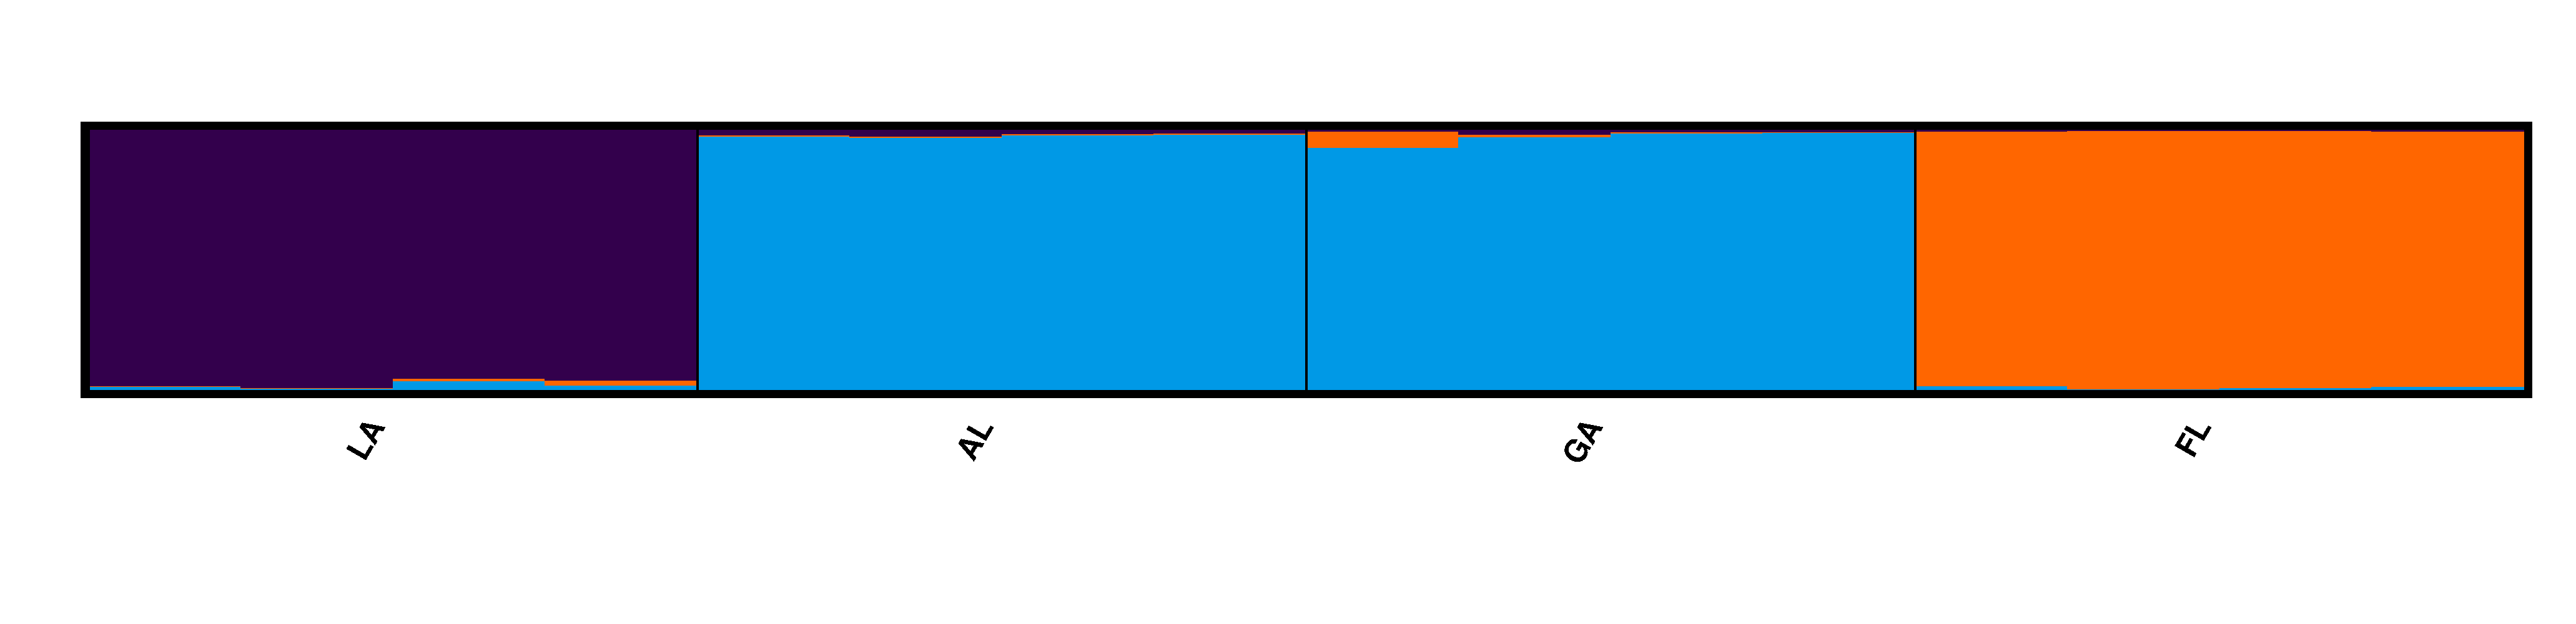
\includegraphics [scale=1.0]{K3MajorCluster}
\noindent
\textbf{Fig. S5} \texttt{STRUCTURE} plot for the partial microsatellite dataset (16 \textit{Gopherus polyphemus} genotyed at 10 microsatellite loci) with optimum number of clusters \textit{K} = 3 determined by \texttt{STRUCTURE HARVESTER}.\\

\pagebreak{}
\noindent
\begin{knitrout}
\definecolor{shadecolor}{rgb}{0.969, 0.969, 0.969}\color{fgcolor}
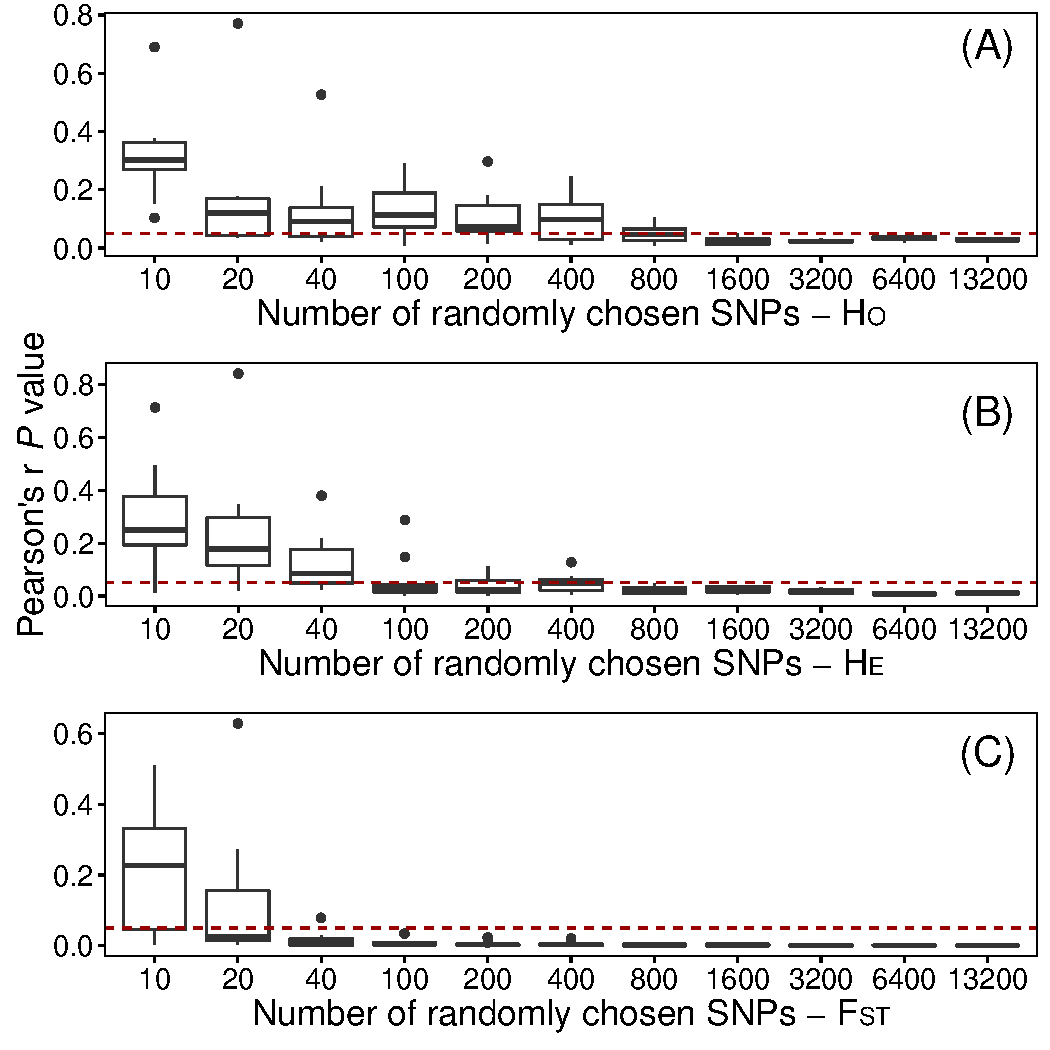
\includegraphics[width=\maxwidth]{figure/Figure-S6-1} 

\end{knitrout}
\noindent
\textbf{Fig. S6} Subsampling analysis showing how many randomly sampled SNP loci out of the total of 17,901 are needed in comparison to the full microsatellite dataset (101 \textit{Gopherus polyphemus} genotyed at 10 microsatellite loci) for Pearon's r correlation coefficient to be significant at 0.05 level (dotted line) for (A) observed heterozygosity; (B) expected heterozygosity; and (C) \textsc{Fst}. There were 10 simulations for each size class of SNPs. \textsc{Ho} for observed heterozygosity, \textsc{He} for expected heterozygosity.\\

\pagebreak{}
\noindent
\begin{knitrout}
\definecolor{shadecolor}{rgb}{0.969, 0.969, 0.969}\color{fgcolor}
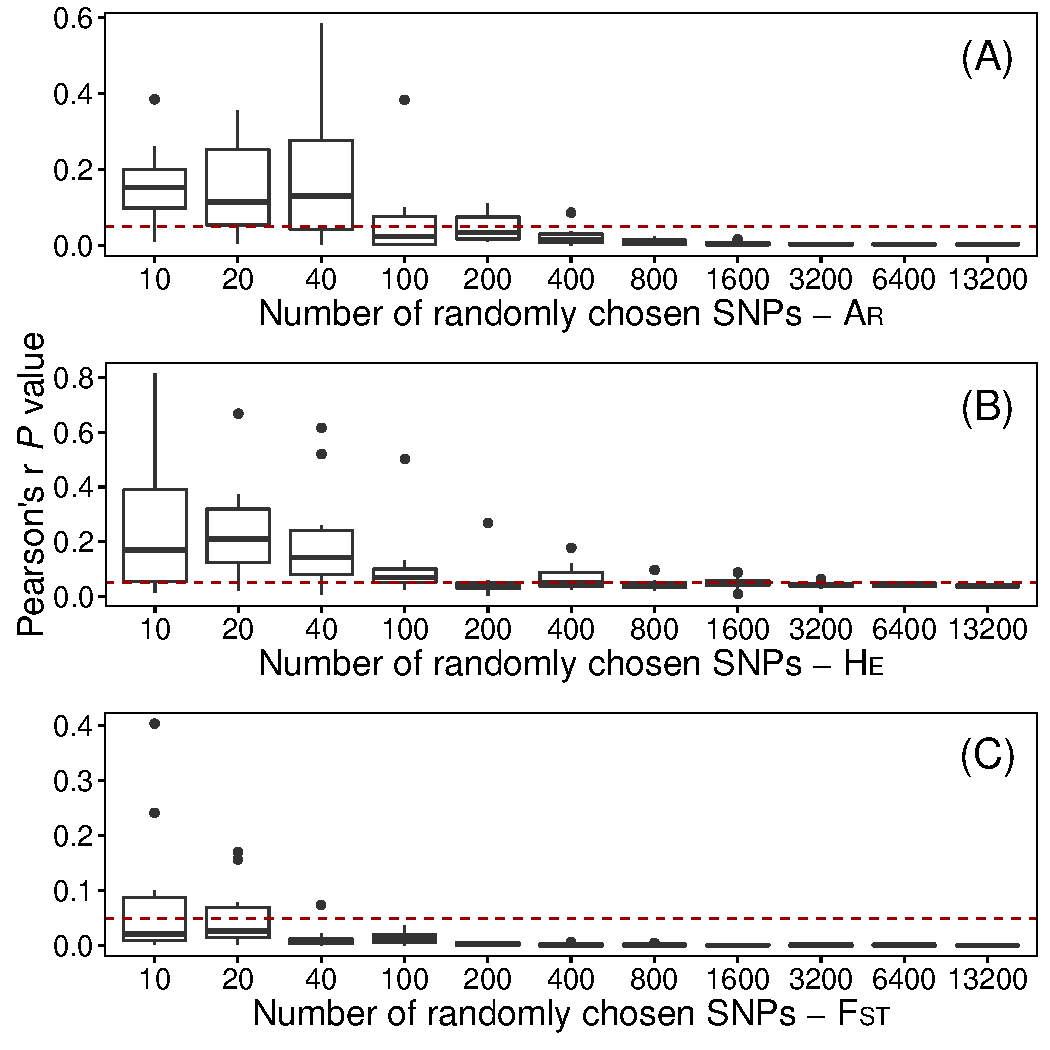
\includegraphics[width=\maxwidth]{figure/Figure-S7-1} 

\end{knitrout}
\noindent
\textbf{Fig. S7} Subsampling analysis showing how many randomly sampled SNP loci out of the total of 17,901 are needed in comparison to the partial microsatellite dataset (16 \textit{Gopherus polyphemus} genotyed at 10 microsatellite loci) for Pearon's r correlation coefficient to be significant at 0.05 level (dotted line) for (A) allelic richness; (B) expected heterozygosity; and (C) \textsc{Fst}. There were 10 simulations for each size class of SNPs. \textsc{Ar} for allelic richness, \textsc{He} for expected heterozygosity.\\ 


\begin{knitrout}
\definecolor{shadecolor}{rgb}{0.969, 0.969, 0.969}\color{fgcolor}
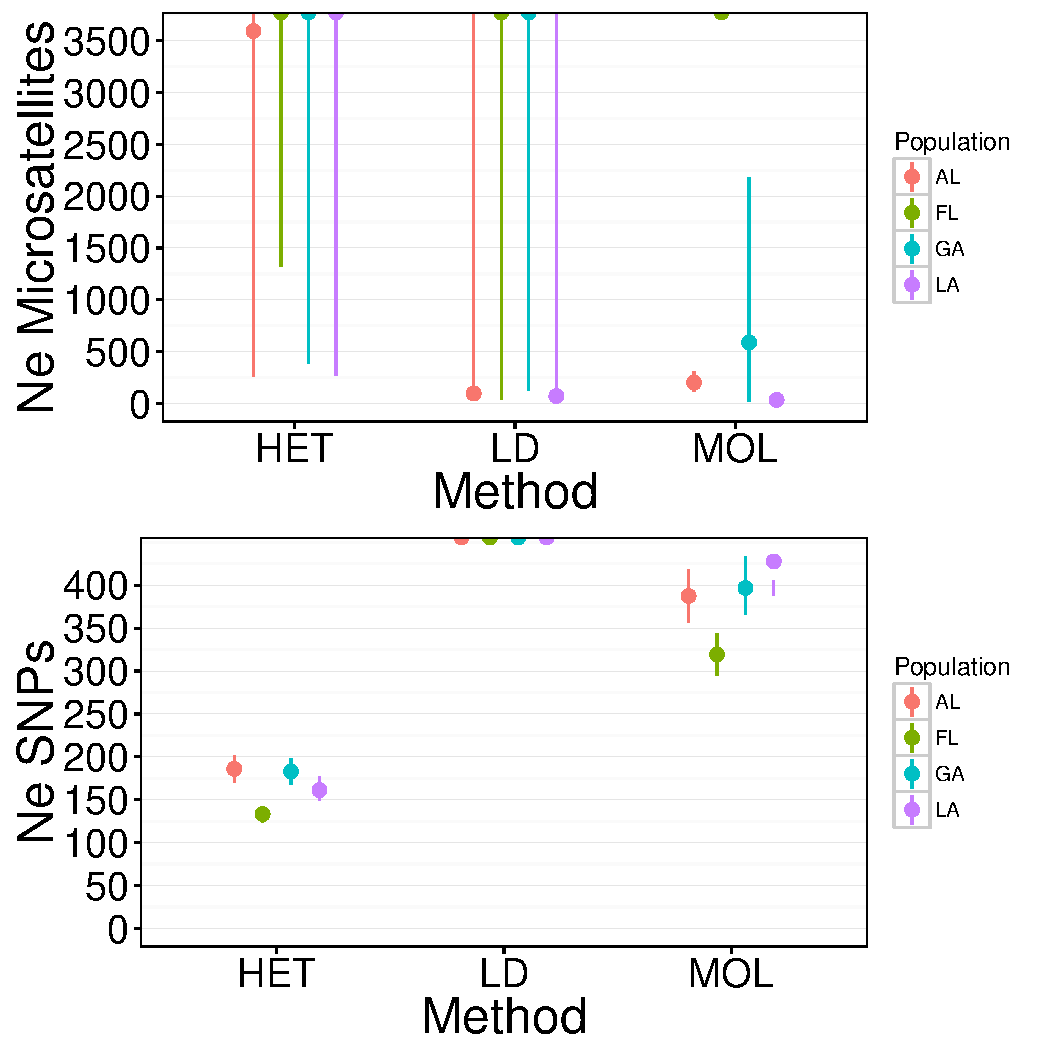
\includegraphics[width=\maxwidth]{figure/Figure_S8-1} 

\end{knitrout}
\noindent
\textbf{Fig. S8} Effective population sizes per generation (Ne) along with 95 \% confidence intervals for \textit{Gopherus polyphemus} samples estimated with the program \texttt{NeEstimator} using (A) the full microsatellite dataset (101 \textit{G. polyphemus} genotyed at 10 microsatellite loci) or (B) the SNP dataset (16 \textit{G. polyphemus} sequenced at 17,901 immune gene SNPs). Dots that are on the top of the graph represent Ne estimates of infinity, and lines that extend to the top of the graph represent upper 95 \% confidence limits of infinity. LD for linkage disequilibrium method of Waples \& Do (2008), HET for heterozygote-excess method of Zhdanova \& Pudovkin (2008), and MOL for the molecular coancestry method of Nomura (2008). Note that the HET and MOL methods estimate the effective number of breeders per year (Nb), which were converted to Ne by multiplying Nb by the generation time of 31 years for \textit{G. polyphemus} (Enge et al. 2006).\\

\end{document}
